\chapter{シミュレーション実験}\label{chap:simulation_experiment}

\section{はじめに}
本章では, 3章にて提案した手法をMCLに実装し, 
4.5節でシミュレータ環境にて, 提案した手法実装したMCLによる実験結果を示す. 
4.6節にて本章をまとめる. 

\section{環境}

\subsection{シミュレータ環境}

提案したアルゴリズムを評価するために図\ref{fig:sim_world}のような
シミュレータ環境を用いた. 図\ref{fig:sim_world}の環境は図\ref{fig:unknown-obstacles}
の実環境を模したものであり, 図\ref{fig:known-obstacles}の2次元マップを
縦方向に伸ばすことによって作成した3次元の環境である. 
シミュレータ環境内で使用したロボットは, 
Raspberry Pi Cat(以下ラズパイキャット)をモデリングしたものである. 

\subsection{開発環境}
シミュレータの実行および提案手法の実装を行うに当たって使用したノートPCの
開発環境を表\ref{tabule:pc_spec_sim}にまとめる. 

\begin{table}[ht]
  \caption{開発環境}
  \label{tabule:pc_spec_sim}
  \begin{center}
    \begin{tabular}{l|c} 
      \thline
      ノートPC& \\
      \hline
      CPU & i7-8665U 1.90GHz×8 \\
      GPU & Quadro P520 \\
      RAM & 32GB  \\
      OS & Ubuntu 18.04 LTS \\
      ROS Distributions & Melodic Morenia \\ 
      \thline
    \end{tabular}
  \end{center}
\end{table}


\begin{figure}[h]
  \begin{center}
    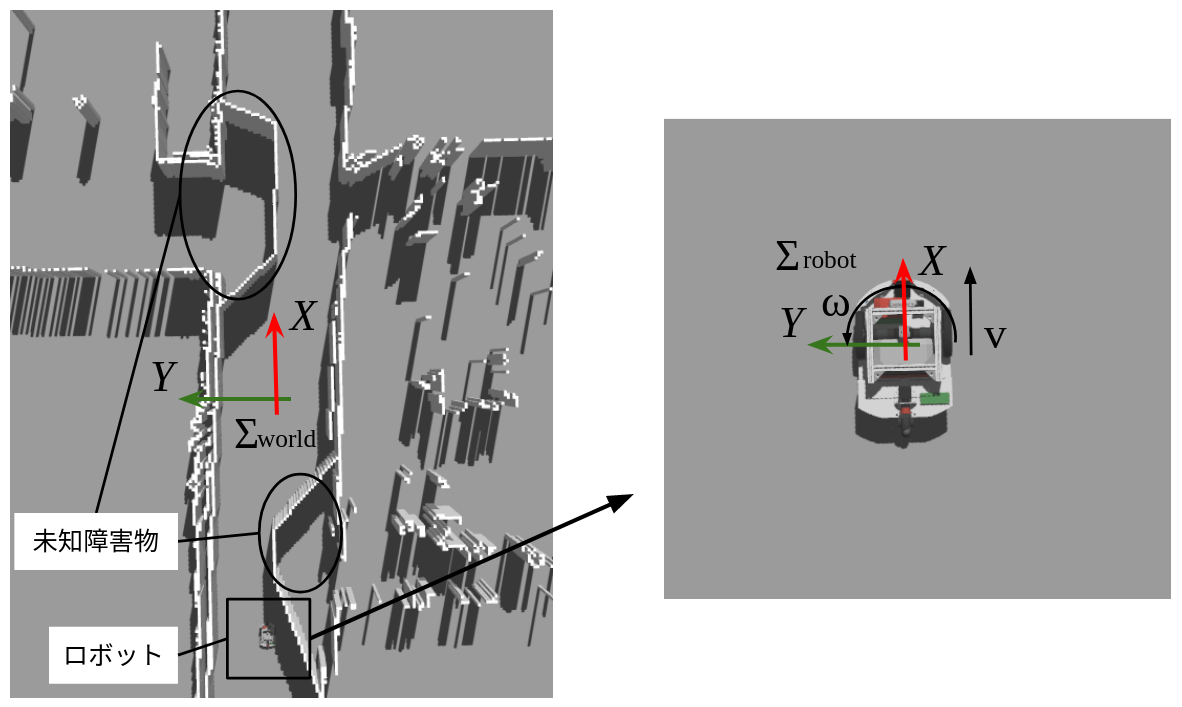
\includegraphics[width=0.98\linewidth]{figs/sim_world.png}
    \caption{使用したシミュレータ環境とロボット}
    \label{fig:sim_world_experiment}
  \end{center}
\end{figure}

\newpage

\begin{figure}[H]
  \begin{center}
    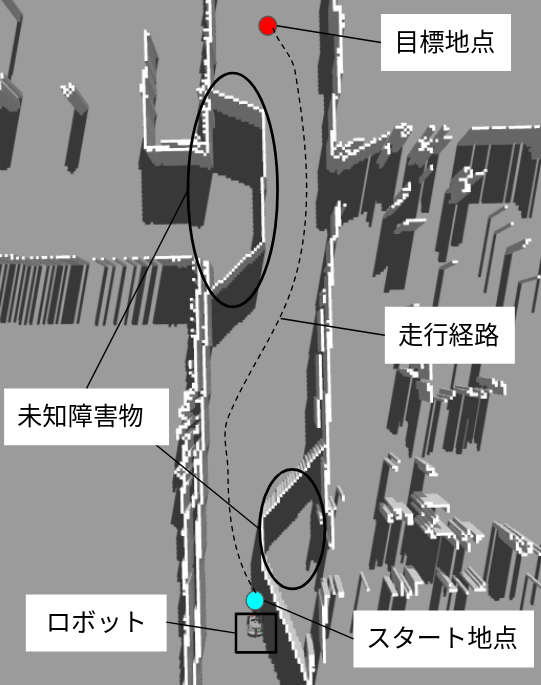
\includegraphics[width=0.5\linewidth]{figs/gazebo_unknown_obstacles.png}
    \caption{スタートと目標地点}
    \label{fig:start_goal_sim}
  \end{center}
\end{figure}

\section{MCLに提案した手法の実装}

提案したアルゴリズムを実装する基になるパッケージとして, 自己位置推定用
のROSパッケージとして公開されているemclを用いる. 
このemclをフォーク[????]して, thesisというブランチで実装を行った. 
実装後のコミット番号はfbb1d9fであり, このコミット番号まで実装した内容について説明していく. 

emclでは, オブジェクト指向を基に, パーティクルフィルタに必要な関数が複数のファイルにて
実装されており, emcl\_node.cpp内でそれらの関数の呼び出しを行っている. 
まず, ExpResetMcl.cppに観測パターンを用意するための関数(generateScanPattern, randomScan)を実装した. 
その関数は, パーティクルの初期化と同時に各パーティクルに対して
図\ref{fig:1}のようなランダムな観測パターンを与える. 
次に, リサンプリング時に, ある観測パターンに収束し続けないように, 全パーティクルのうち$10\%$
のパーティクルをサンプルし, ランダムな観測パターンをそれぞれに与える実装を行った. 

\section{実験方法}

図\ref{fig:sim_world_experiment}のシミュレータ環境用いて, 提案したアルゴリズムを実装したemclの評価を行う. 
実験では未知障害物がある環境を走行した場合において, 以下の項目について評価を行う. 
\begin{itemize}
  \item 走行の評価
  \item 推定された自己位置
  \item 自己位置の尤度
  \item 使用された観測パターン
  \item 尤度計算にかかった時間
\end{itemize}
4.5.1では提案した手法の実装が無い, 4.5.2では提案した手法の実装がある場合において, 
未知障害物が存在するシミュレータ環境で自律走行をした時の評価をまとめる. 

\newpage

\section{実験結果}

\subsection{提案した手法の実装無し}

図\ref{fig:nav_no_imp}のように, 未知障害物が存在するシミュレータ環境において, 提案した手法の実装が無いリセット付きの自己位置推定の場合, 
目標地点にたどり着くことができなかった. これは, 奥側にある未知障害物によって, リセットがかかり続けたため, 
自己位置推定が破綻してしまったことが原因である. 

\begin{figure}[H]
  \begin{center}
    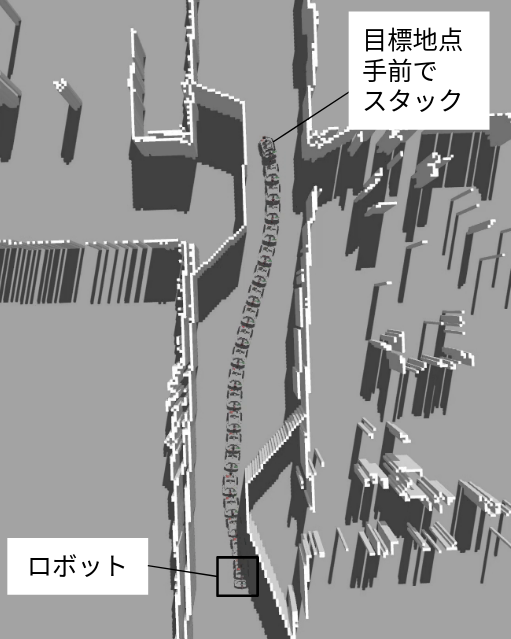
\includegraphics[width=0.5\linewidth]{figs/no_implementation_with_reset.png}
    \caption{未知障害物があるシミュレータ環境での自律走行(提案手法の実装無し)}
    \label{fig:nav_no_imp}
  \end{center}
\end{figure}

自律走行時のロボットの位置の真値と
走行中に推定された自己位置と比較したグラフは, 図\ref{fig:odom_comp_no_imp}のようになった. 
奥側の未知障害物を走行している20秒辺りでは, 推定された自己位置とロボットの位置の真値として
, x, y方向ともに誤差が生じており, 特にy方向の誤差が大きくなってしまっている. 
これは, 未知障害物によって, 何度もリセットがかかり続けてしまったため, 自己位置推定が不確かになってしまったといえる. 

\begin{figure}[H]
  \begin{center}
    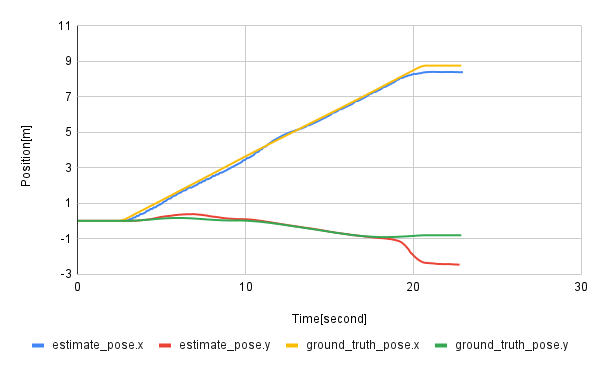
\includegraphics[width=0.98\linewidth]{figs/sim_no_imp_ground_truth.png}
    \caption{推定された自己位置とロボットの位置の真値との比較}
    \label{fig:odom_comp_no_imp}
  \end{center}
\end{figure}

自律走行時の尤度は, 図\ref{fig:nav_likelihood_no_imp}のようになった. 
未知障害物付近を走行している5秒, 20秒辺りでは, ともに尤度が著しく低下してしまっている. 

\begin{figure}[H]
  \begin{center}
    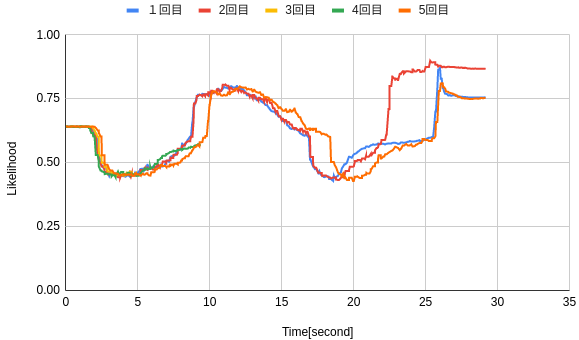
\includegraphics[width=0.98\linewidth]{figs/sim_likelihood_before.png}
    \caption{自律走行時の自己位置の尤度}
    \label{fig:nav_likelihood_no_imp}
  \end{center}
\end{figure}

提案手法の実装が無い場合において, スタートから目標地点までの走行の際に, 
尤度計算にかかった時間は表\ref{tabule:likelihood_calc_time_sim_no_imp}のとおりになった. 

\begin{table}[ht]
  \begin{center}
    \caption{提案手法の実装が無い場合の実験結果}
    \label{tabule:likelihood_calc_time_sim_no_imp}
    \begin{tabular}{l|r|r} 
      \thline
      & 平均[ms] &  標準偏差[ms] \\
      \hline
      尤度計算にかかった時間 & 34.09 & 13.02 \\
      \thline
    \end{tabular}
  \end{center}
\end{table}

\subsection{提案した手法の実装あり}

提案した手法の実装があるリセット付きの自己位置推定では, 目標地点に到達することができた. 

\begin{figure}[H]
  \begin{center}
    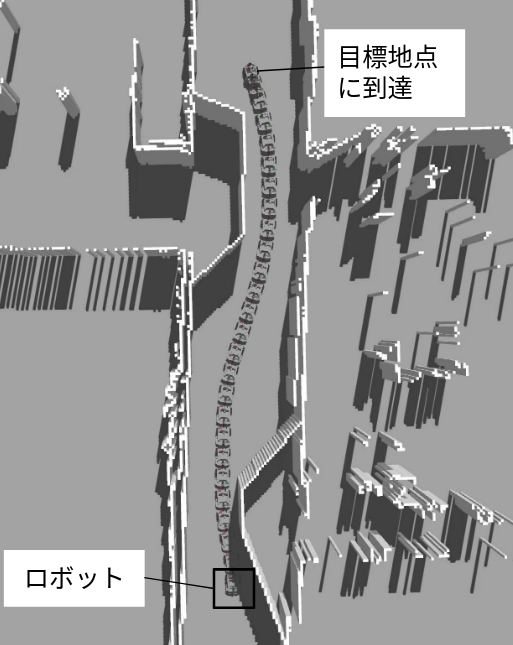
\includegraphics[width=0.5\linewidth]{figs/no_implementation_no_reset.png}
    \caption{未知障害物があるシミュレータ環境での自律走行(提案手法の実装あり)}
    \label{fig:nav_imp}
  \end{center}
\end{figure}

自律走行時のロボットの位置の真値と
走行中に推定された自己位置と比較したグラフは, 図\ref{fig:odom_comp_imp}のようになった. 
推定された自己位置とロボットの位置の真値を比較して, 目立った誤差はないといえる. 

\begin{figure}[H]
  \begin{center}
    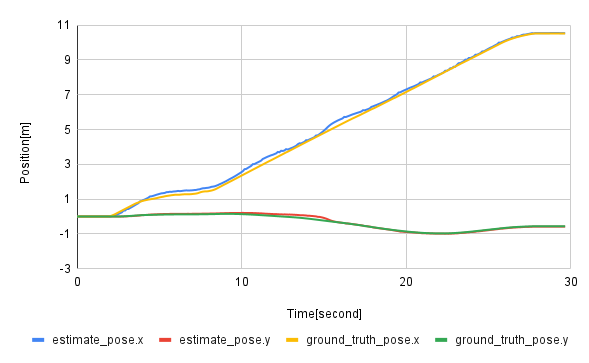
\includegraphics[width=0.98\linewidth]{figs/sim_imp_ground_truth.png}
    \caption{推定された自己位置とロボットの位置の真値との比較}
    \label{fig:odom_comp_imp}
  \end{center}
\end{figure}

自律走行時の尤度は, 図\ref{fig:nav_likelihood_imp}のようになった. 
未知障害物付近の走行時において, 尤度は著しく低下することなく, 安定していることがわかる. 

\begin{figure}[H]
  \begin{center}
    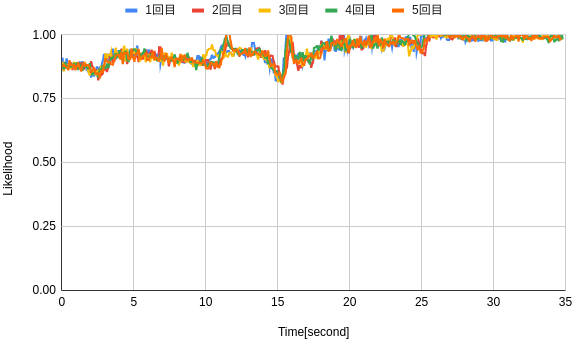
\includegraphics[width=0.98\linewidth]{figs/sim_likelihood_after.png}
    \caption{自律走行時の自己位置の尤度}
    \label{fig:nav_likelihood_imp}
  \end{center}
\end{figure}

自律走行時において, パーティクルの中で最も使用された観測パターンを表したグラフは
図\ref{fig:obs_pattern_sim}のようになった. 
グラフからは, 未知障害物に応じて観測パターンを選択できていることがわかる. 

\begin{figure}[h]
  \begin{center}
    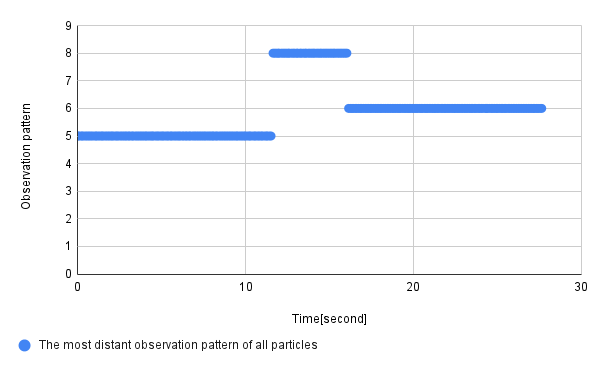
\includegraphics[width=0.98\linewidth]{figs/sim_imp_ob_pattern.png}
    \caption{自律走行時にパーティクルの中で最も使用された観測パターン}
    \label{fig:obs_pattern_sim}
  \end{center}
\end{figure}

提案手法の実装がある場合において, スタートから目標地点までの走行の際に, 
尤度計算にかかった時間は表\ref{tabule:likelihood_calc_time_sim_imp}のとおりになった. 

\begin{table}[ht]
  \begin{center}
    \caption{提案手法の実装がある場合の実験結果}
    \label{tabule:likelihood_calc_time_sim_imp}
    \begin{tabular}{l|r|r} 
      \thline
      & 平均[ms] &  標準偏差[ms] \\
      \hline
      尤度計算にかかった時間 & 30.76 & 6.35 \\
      \thline
    \end{tabular}
  \end{center}
\end{table}

\section{まとめ}
未知障害物が存在するシミュレータ環境において, 提案手法の実装がある場合と無い場合の結果を示した. 
実験の結果から、提案手法の実装を行うことで, 未知障害物による影響を受けずに自己位置推定ができることが確認できた. 
また, 提案手法の実装を行うことで, 尤度計算にかかる時間が従来より4[ms]短縮していることも確認できた. 